\documentclass[12pt]{article}
\usepackage{listings}
\usepackage{graphicx}
\usepackage{xcolor}

\begin{document}
\title{ECEC 471 Lab 3}
\author{Nicholas Sica}
\date{October 29, 2020}
\maketitle

\section{Introduction}
\subsection{Overview}
This lab is meant to use the knowledge gained in lab 2 to build a symmetric version of the nand and nor gates.
CMOS circuits are designed by tying the outputs of a pull down and pull up network together. For the nand gate, the pull up network is two pmos transistors in parallel tied to
voltage high, or Vdd, and the pull down network is two nmos transistors in series tied to voltage low, or ground. The nor gate has the pull-up and pull-down networks swapped.
A nand outputs a zero when both inputs are high and a one otherwise, while a nor outputs a zero when either input is high and a zero otherwise.
Rise time and fall time are the time it takes for the ouput to rise from 10\% to 90\% of the total voltage or fall from 90\% to 10\% of the total voltage.
Propagation delay is the time it takes for the output to appear after the input, usually measured by taking the difference of the 50\% marks of the input and output.
\subsection{Symmetric Gates}
A symmetric gate is a gate whose worst case rise and fall times are the same. In other words, the input and output voltage cross the half point of Vdd at the same time. We get a
symmetric gate by keeping the non-worst case path constant and changing the other. The path usually kept constant in simple gate is the path with the parallel transistors, while
the series transistors are changed. This is the pull-down network for the nand and the pull-up network for the nor in this lab.
\section{Simulation and Analysis}
\subsection{NAND Schematic Design}
Figure~\ref{fig:nand_schem} shows the transistor-level schematic of the nand gate after the ideal width for the nmos transistors was found.
The initial width of every transistor in the circuit was 90nm before the change and the length of every transistor in the circuit is 50nm. After the change, the width of the nmos
transistors became 200nm.
\begin{figure}[!htb]
  \centering
  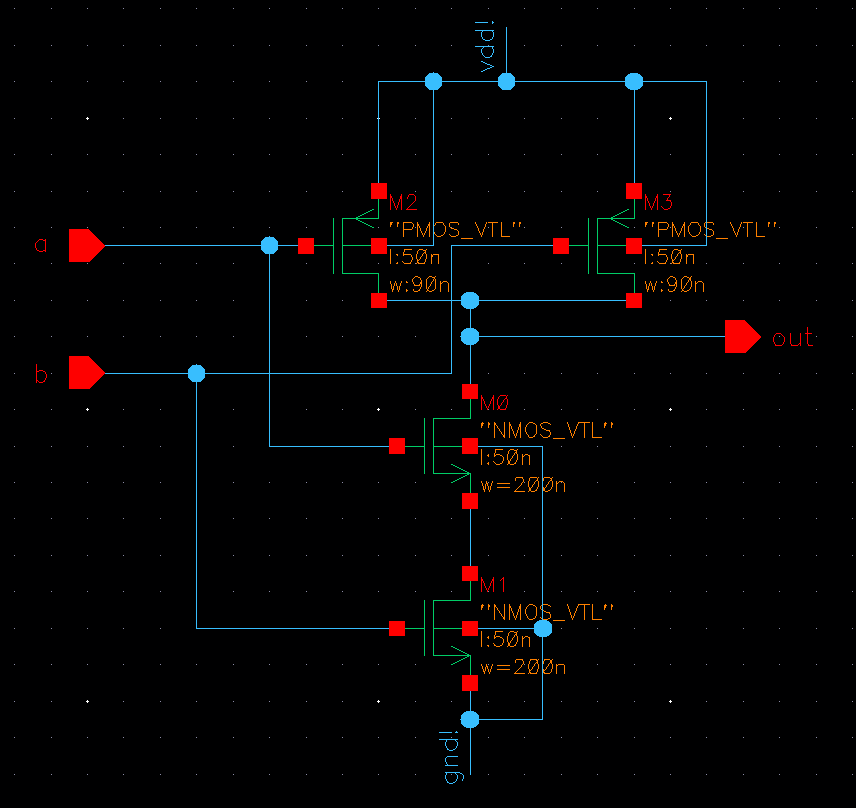
\includegraphics[width=4in]{figures/nand/nand_schem.png}
  \caption{Transistor-level Symmetric NAND Schematic}\label{fig:nand_schem}
\end{figure}
Figure~\ref{fig:nand_sim} shows the simulation schematic with the source and load. A pulse is used so we can measure the rise and fall times as well as the propagation delay. The
pulse has an amplitude of 1.2V, a period of 2ns, a rise time of 5ps, a fall time of 5ps and a pulse width of 1ns. A 5fF capacitor was tied to the output to get it closer to a
realistic model where the output of the nand gate would have some capacitance.
\begin{figure}[!htb]
  \centering
  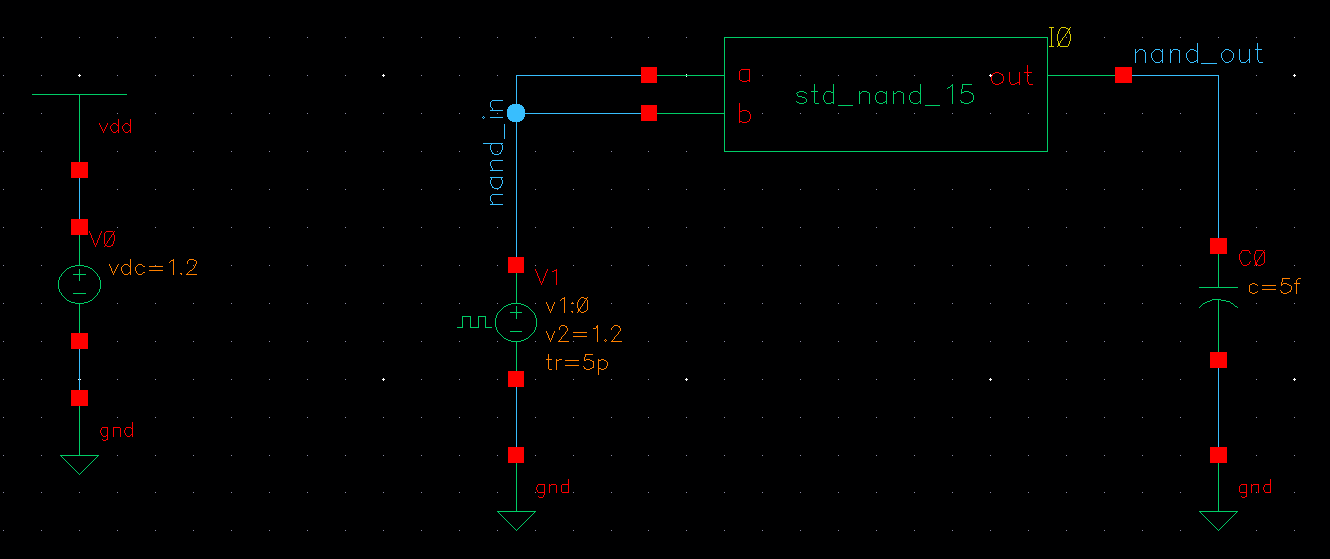
\includegraphics[width=5in]{figures/nand/nand_sim.png}
  \caption{NAND Simulation Schematic}\label{fig:nand_sim}
\end{figure}
The transient analysis and DC response of the circuit are shown in Figure~\ref{fig:nand_tran} and Figure~\ref{fig:nand_dc_asymm} respectively. Using the transient analysis graphs a
rise time of 28.67ps, a fall time of 27.70ps, and propagation delay of 9.49ps were all easily found. The switching voltage was found to be 696.338mV using the DC response graph
which is not the desired 0.6V we want for a symmetric nand gate.
\begin{figure}[!htb]
  \centering
  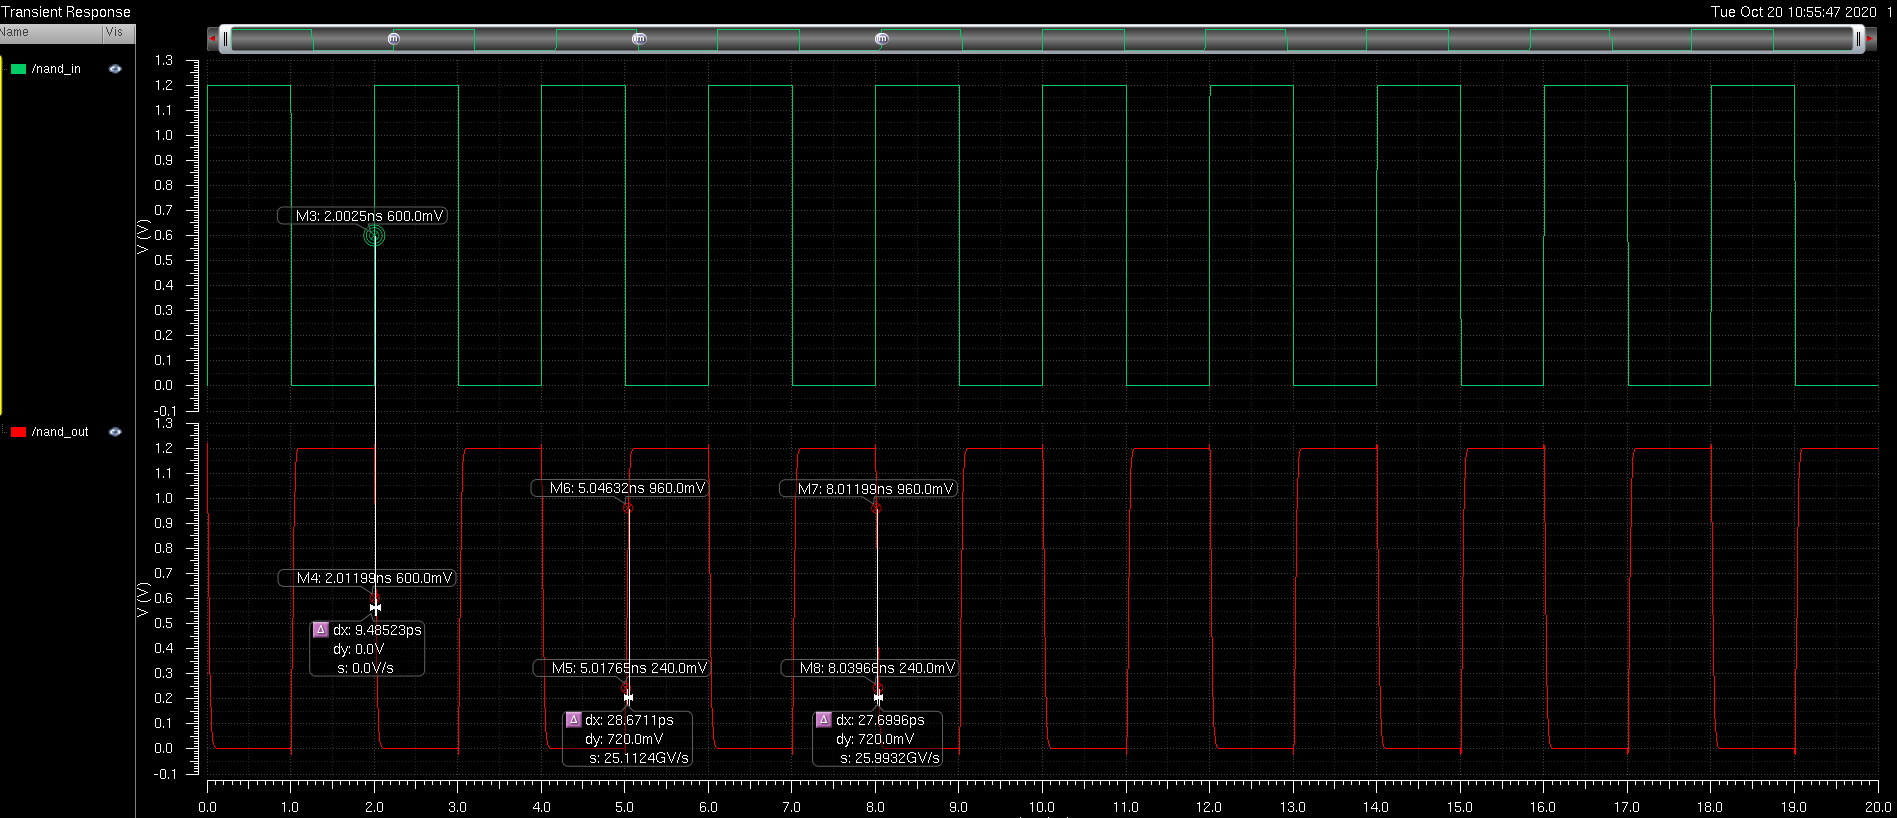
\includegraphics[width=5in]{figures/nand/nand_tran.png}
  \caption{NAND Transient Analysis}\label{fig:nand_tran}
\end{figure}
\begin{figure}[!htb]
  \centering
  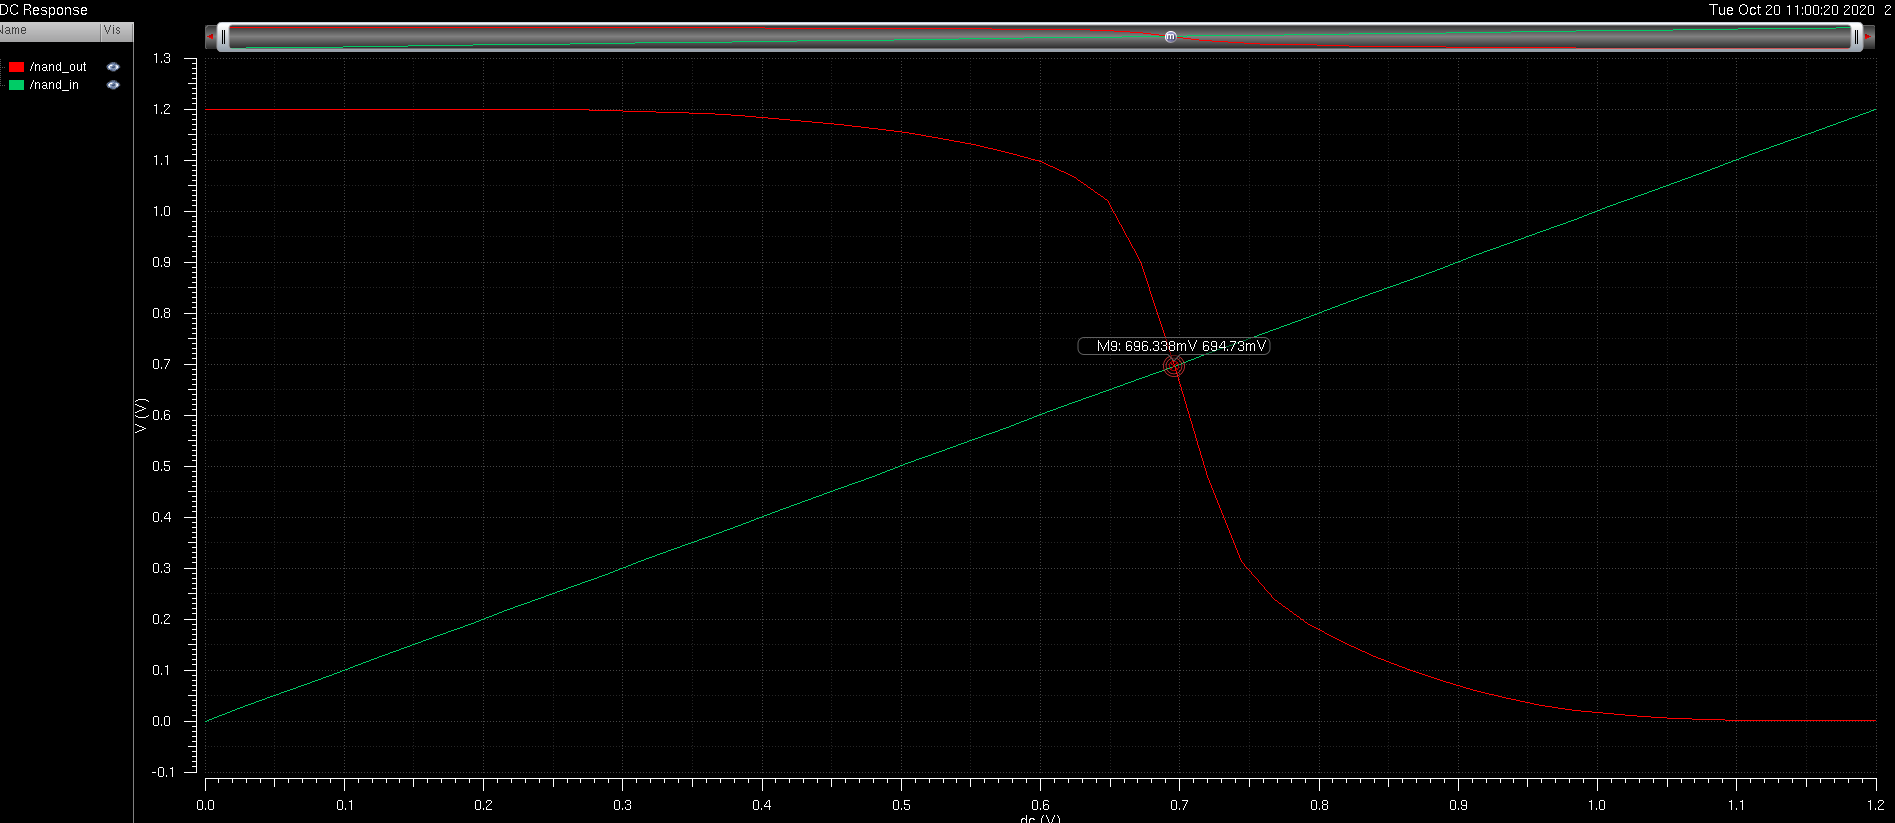
\includegraphics[width=5in]{figures/nand/nand_dc_asymm.png}
  \caption{DC Response of an Asymmetric NAND Gate}\label{fig:nand_dc_asymm}
\end{figure}
To find the desired width of the pmos transistor, we used parametric analysis to get Figure~\ref{fig:nand_param} and found that a width of 200nm gave us a switching voltage of
about 0.6V.
\begin{figure}[!htb]
  \centering
  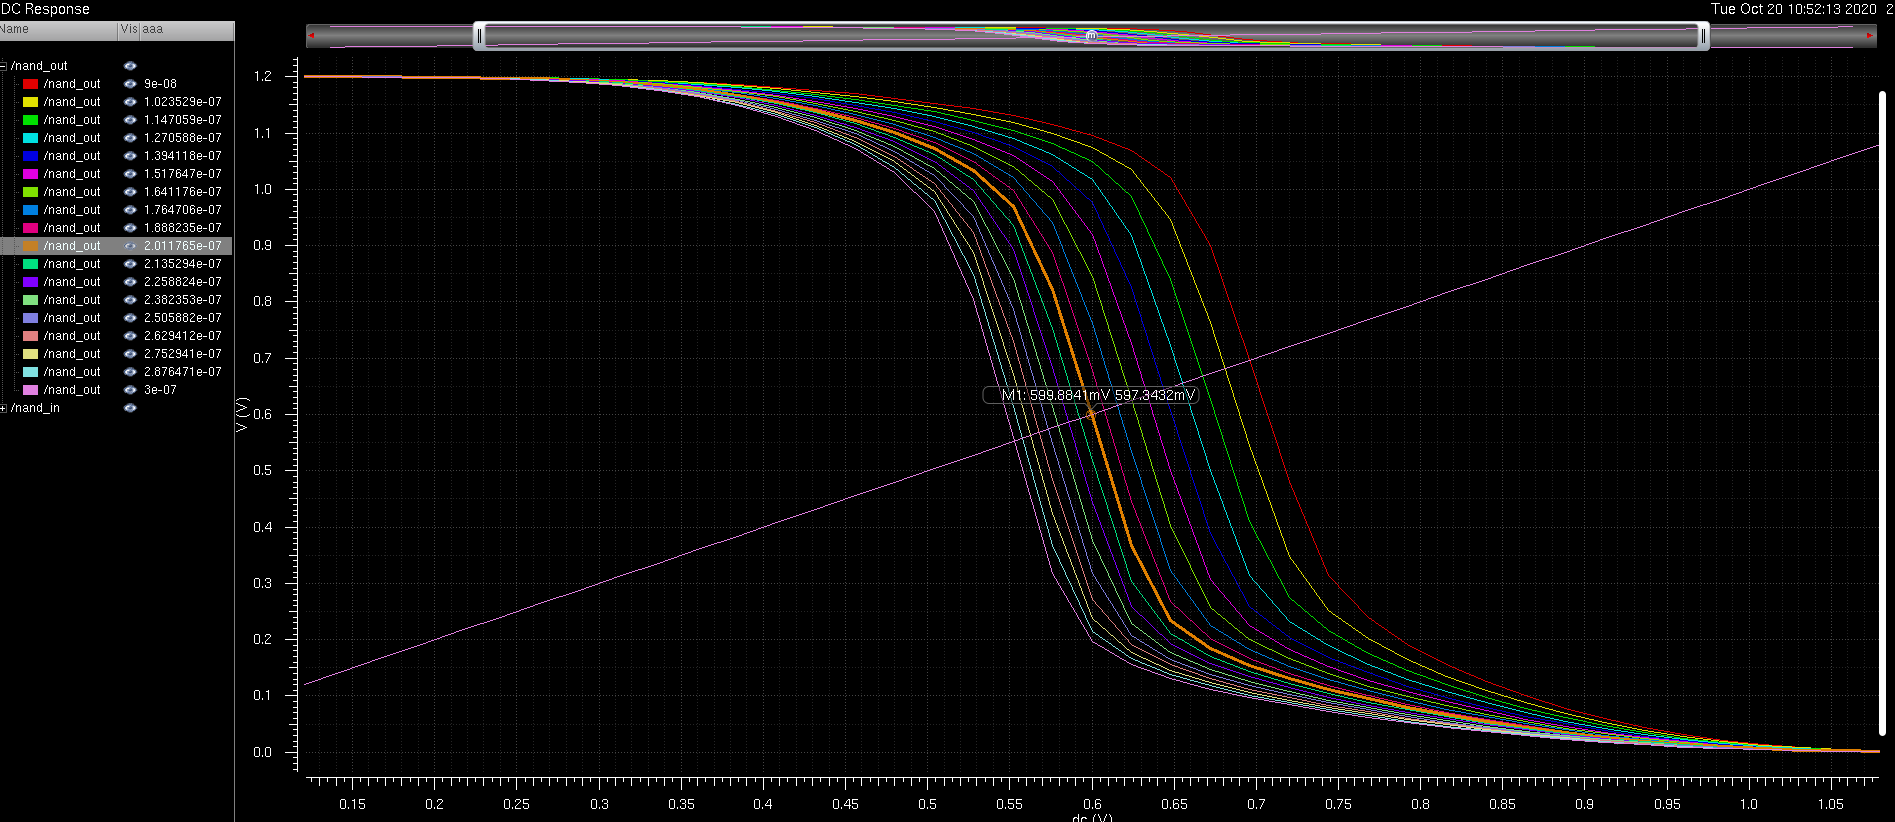
\includegraphics[width=5in]{figures/nand/nand_param.png}
  \caption{NAND Parametric Analysis}\label{fig:nand_param}
\end{figure}
After the schematic was updated to use the new width, DC response was simulated and graphed again to give us Figure~\ref{fig:nand_dc_symm} which shows a switching voltage
of about 0.6V, which is desired.
\begin{figure}[!htb]
  \centering
  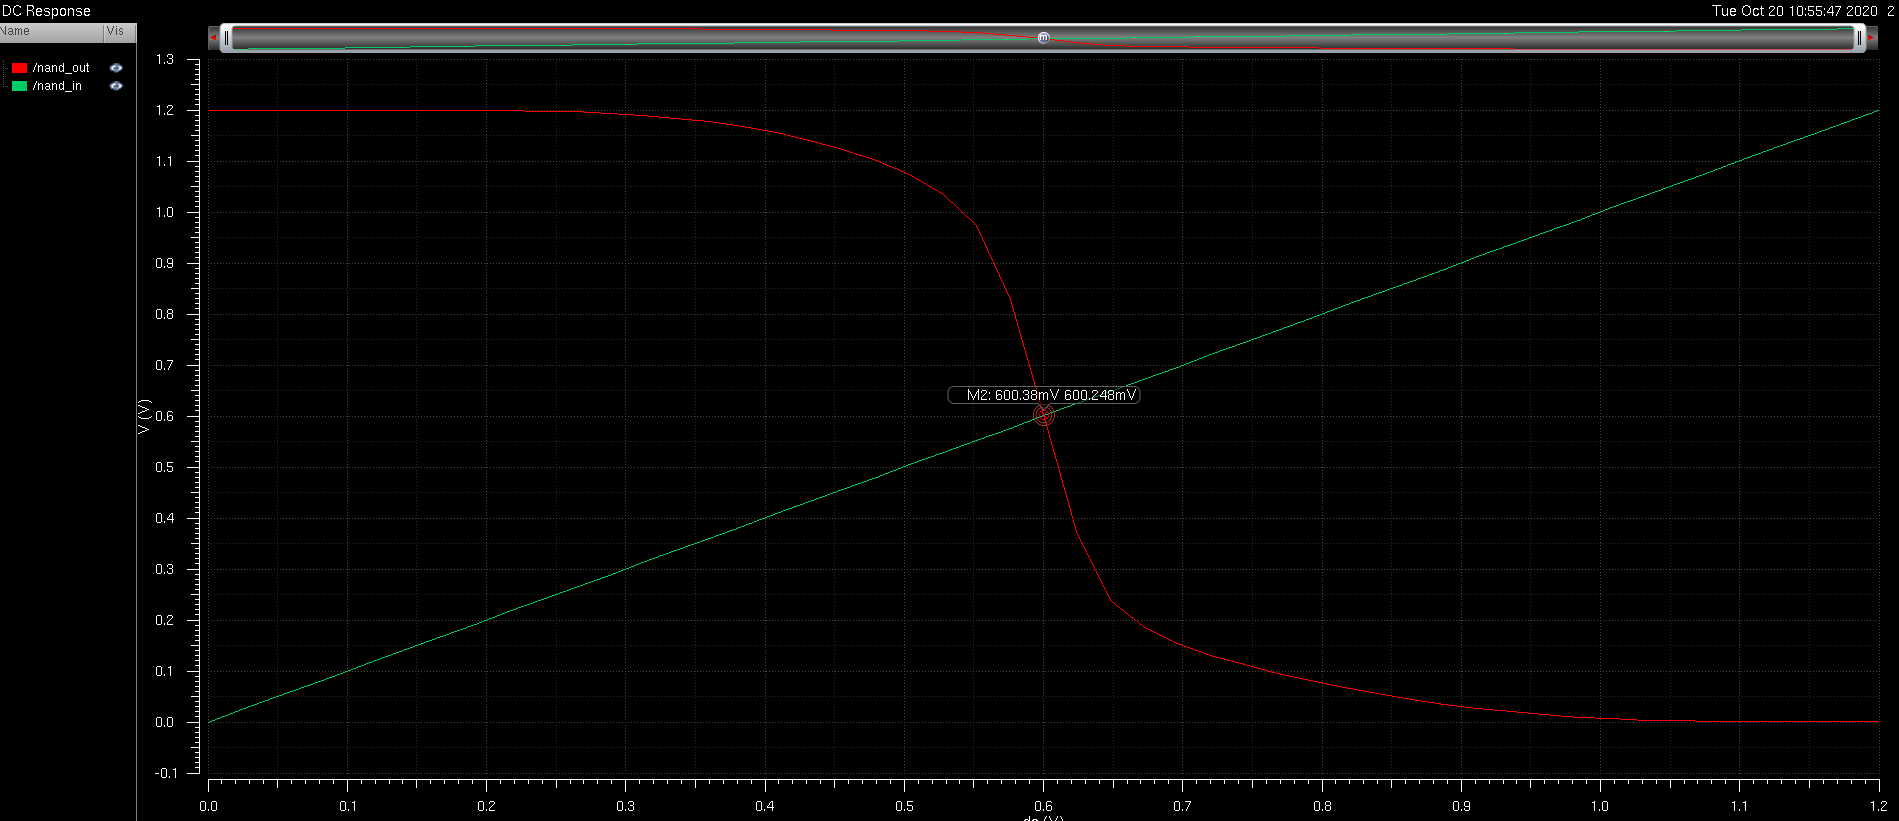
\includegraphics[width=5in]{figures/nand/nand_dc_symm.png}
  \caption{DC Response of a Symmetric NAND Gate}\label{fig:nand_dc_symm}
\end{figure}
\subsection{NOR Schematic Design}
Figure~\ref{fig:nor_schem} shows the transistor-level schematic of the nor gate after the ideal width for the nmos transistors was found.
The initial width of every transistor in the circuit was 90nm before the change and the length of every transistor in the circuit is 50nm. After the change, the width of the nmos
transistors became 547.5nm.
\begin{figure}[!htb]
  \centering
  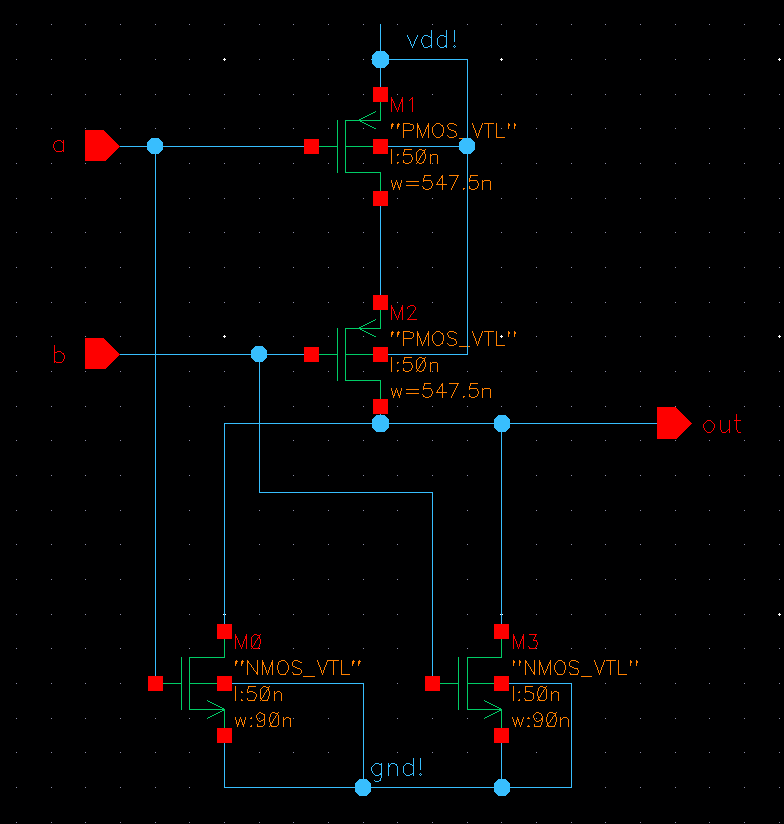
\includegraphics[width=4in]{figures/nor/nor_schem.png}
  \caption{Transistor-level Symmetric NOR Schematic}\label{fig:nor_schem}
\end{figure}
Figure~\ref{fig:nor_sim} shows the simulation schematic with the source and load. A pulse is used so we can measure the rise and fall times as well as the propagation delay. The
pulse has an amplitude of 1.2V, a period of 2ns, a rise time of 5ps, a fall time of 5ps and a pulse width of 1ns. A 5fF capacitor was tied to the output to get it closer to a
realistic model where the output of the nor gate would have some capacitance.
\begin{figure}[!htb]
  \centering
  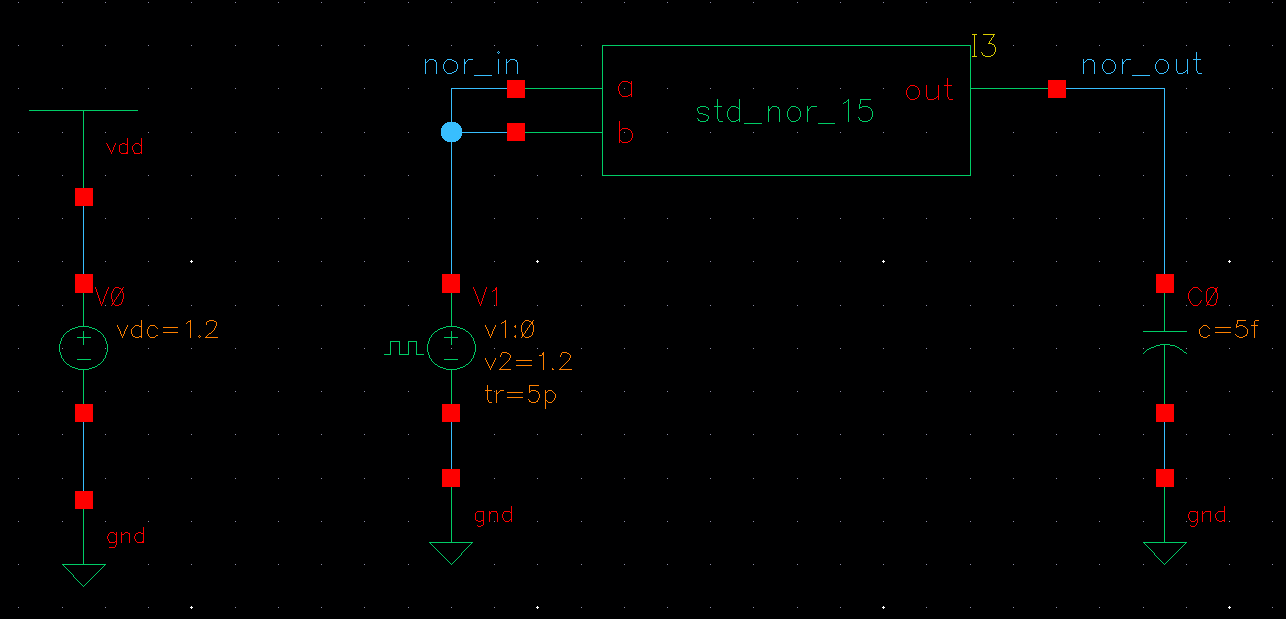
\includegraphics[width=5in]{figures/nor/nor_sim.png}
  \caption{NOR Simulation Schematic}\label{fig:nor_sim}
\end{figure}
The transient analysis and DC response of the circuit are shown in Figure~\ref{fig:nor_tran} and Figure~\ref{fig:nor_dc_asymm} respectively. Using the transient analysis graphs a
rise time of 98.88, a fall time of 17.99ps, and propagation delay of 13.70ps were all easily found. The switching voltage was found to be 412.29mV using the DC response graph
which is not the desired 0.6V we want for a symmetric nor gate.
\begin{figure}[!htb]
  \centering
  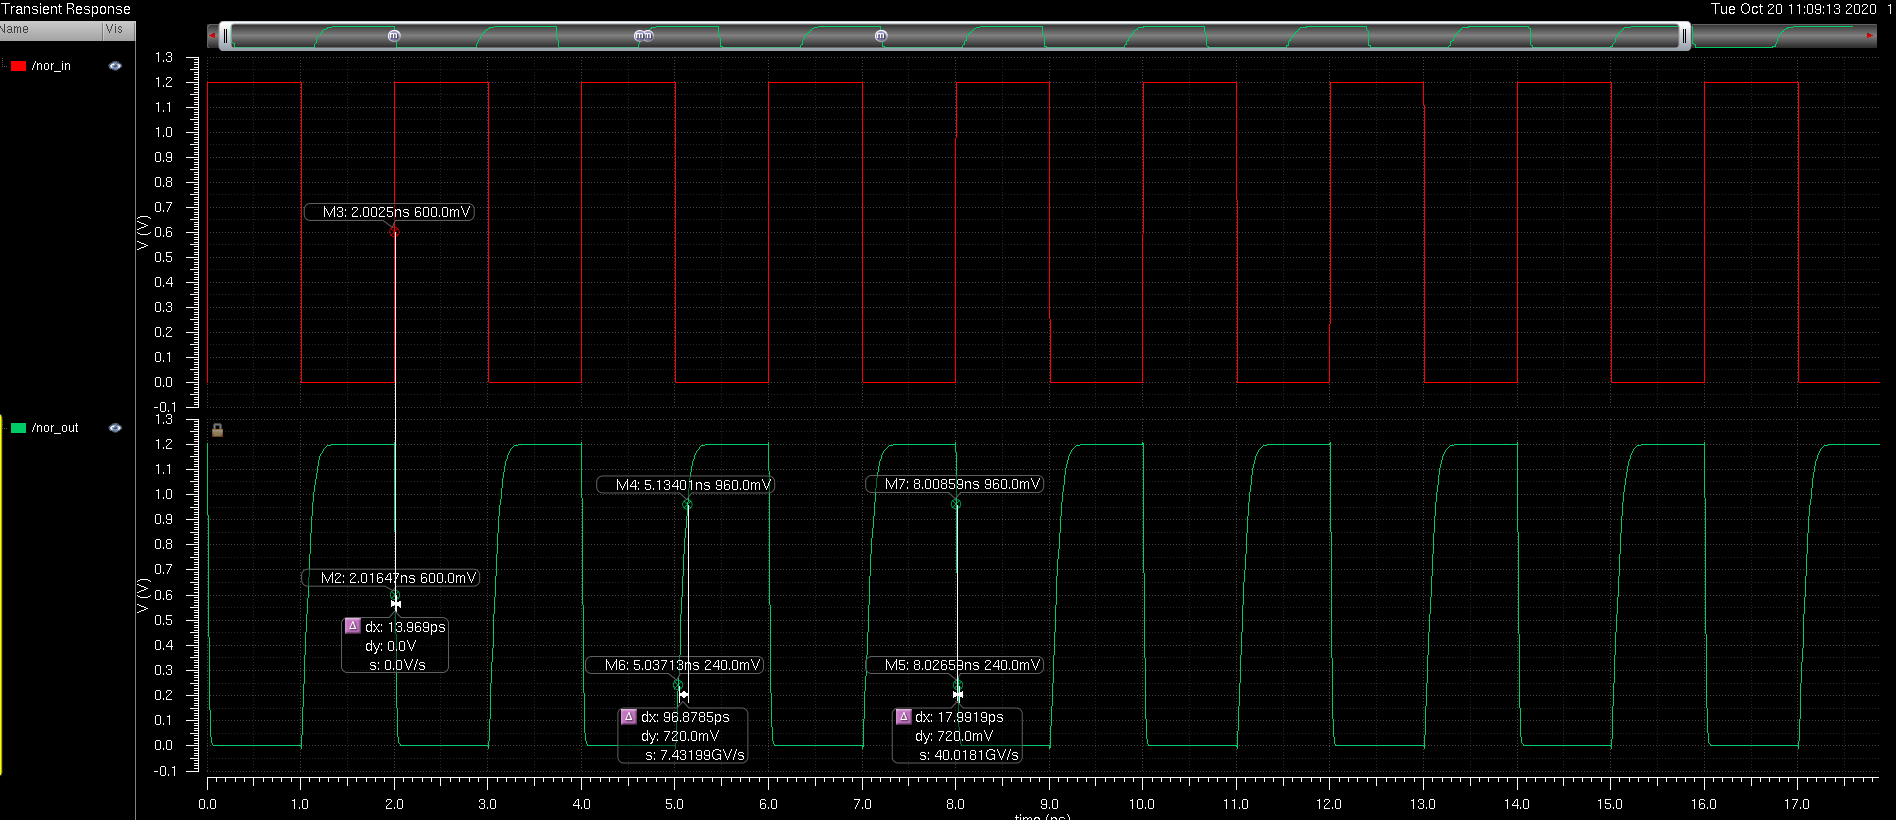
\includegraphics[width=5in]{figures/nor/nor_tran.png}
  \caption{NOR Transient Analysis}\label{fig:nor_tran}
\end{figure}
\begin{figure}[!htb]
  \centering
  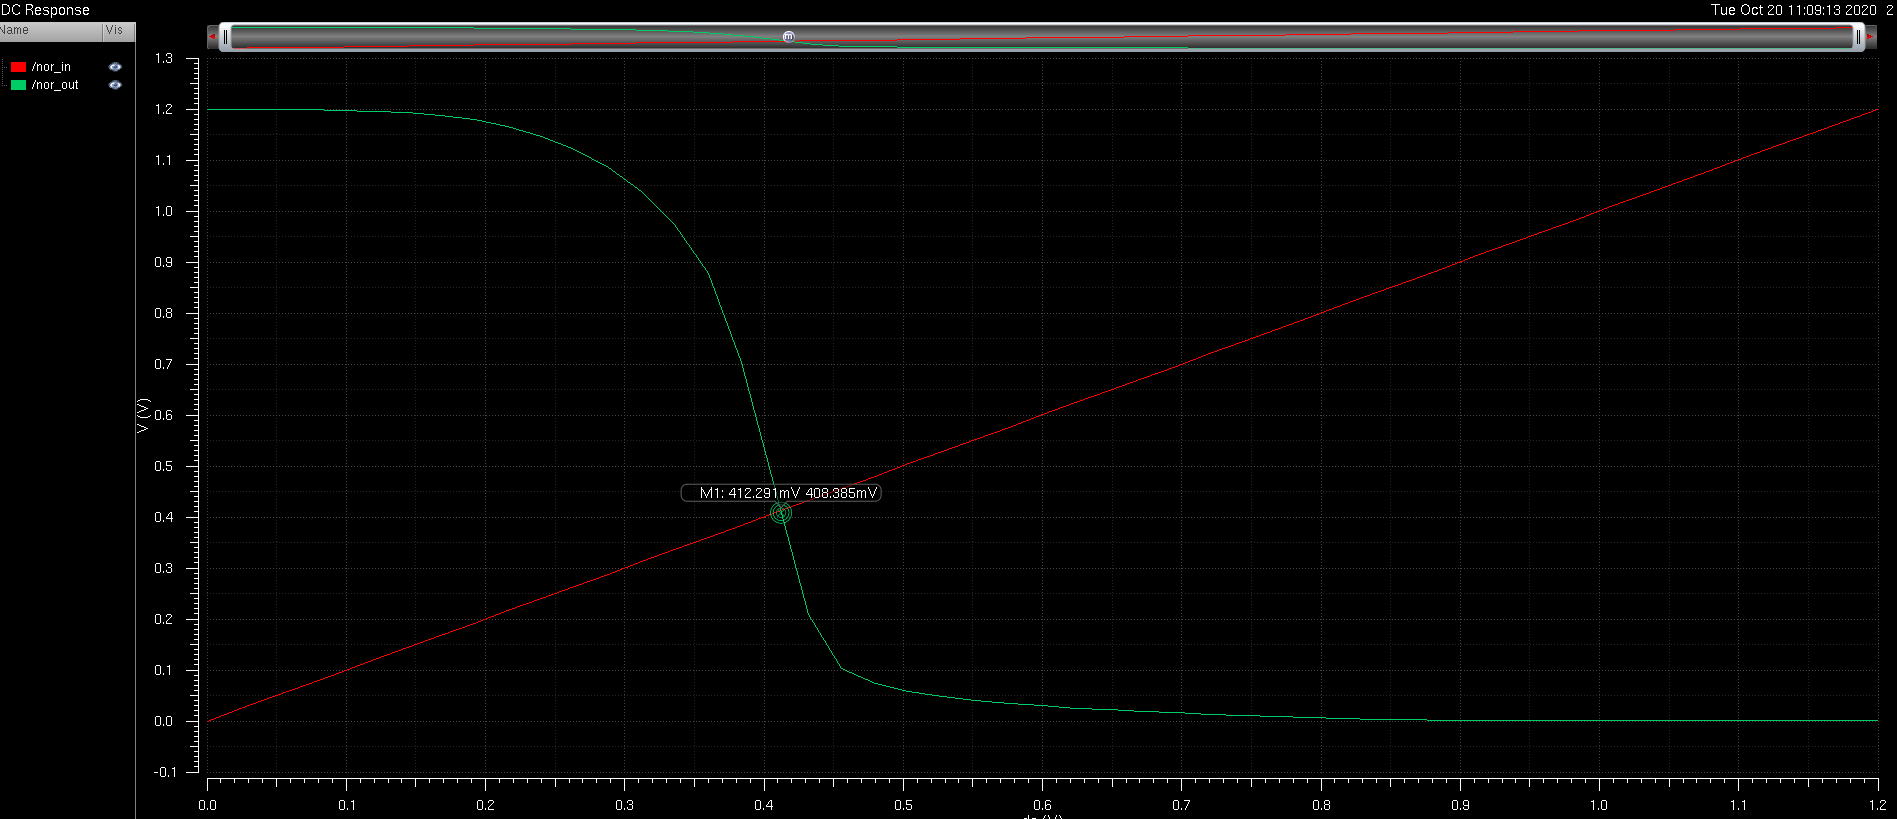
\includegraphics[width=5in]{figures/nor/nor_dc_asymm.png}
  \caption{DC Response of an Asymmetric NOR Gate}\label{fig:nor_dc_asymm}
\end{figure}
To find the desired width of the pmos transistor, we used parametric analysis to get Figure~\ref{fig:nor_param} and found that a width of 547.5nm gave us a switching voltage of
about 0.6V.
\begin{figure}[!htb]
  \centering
  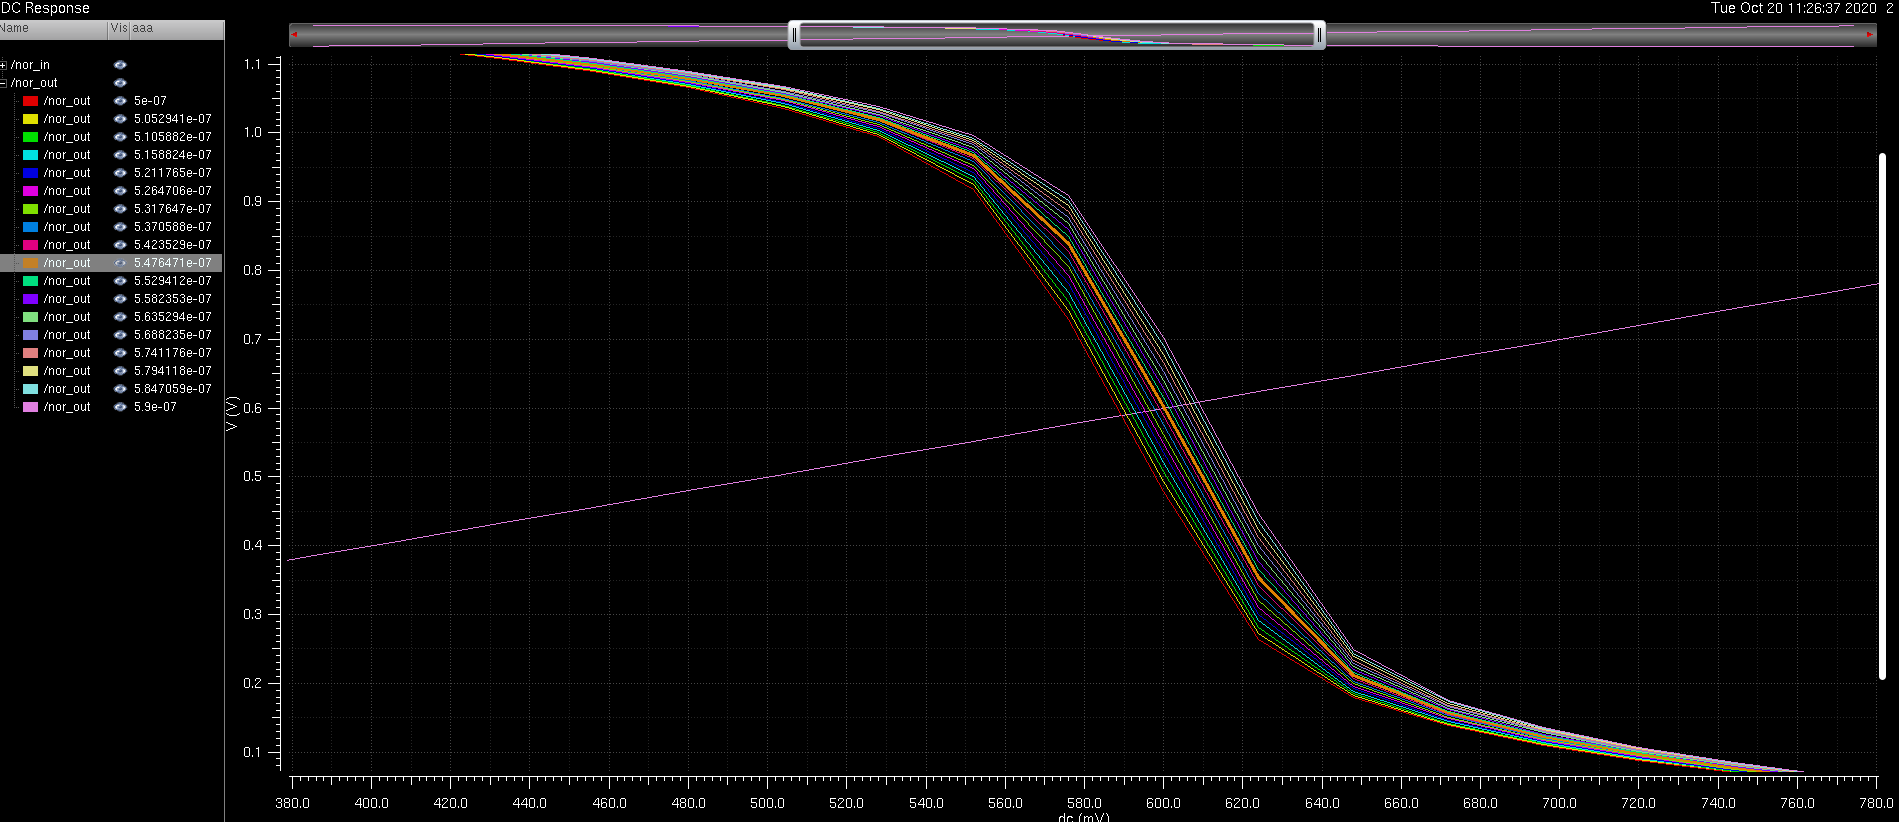
\includegraphics[width=5in]{figures/nor/nor_param.png}
  \caption{NOR Parametric Analysis}\label{fig:nor_param}
\end{figure}
After the schematic was updated to use the new width, DC response was simulated and graphed again to give us Figure~\ref{fig:nor_dc_symm} which shows a switching voltage
of about 0.6V, which is desired.
\begin{figure}[!htb]
  \centering
  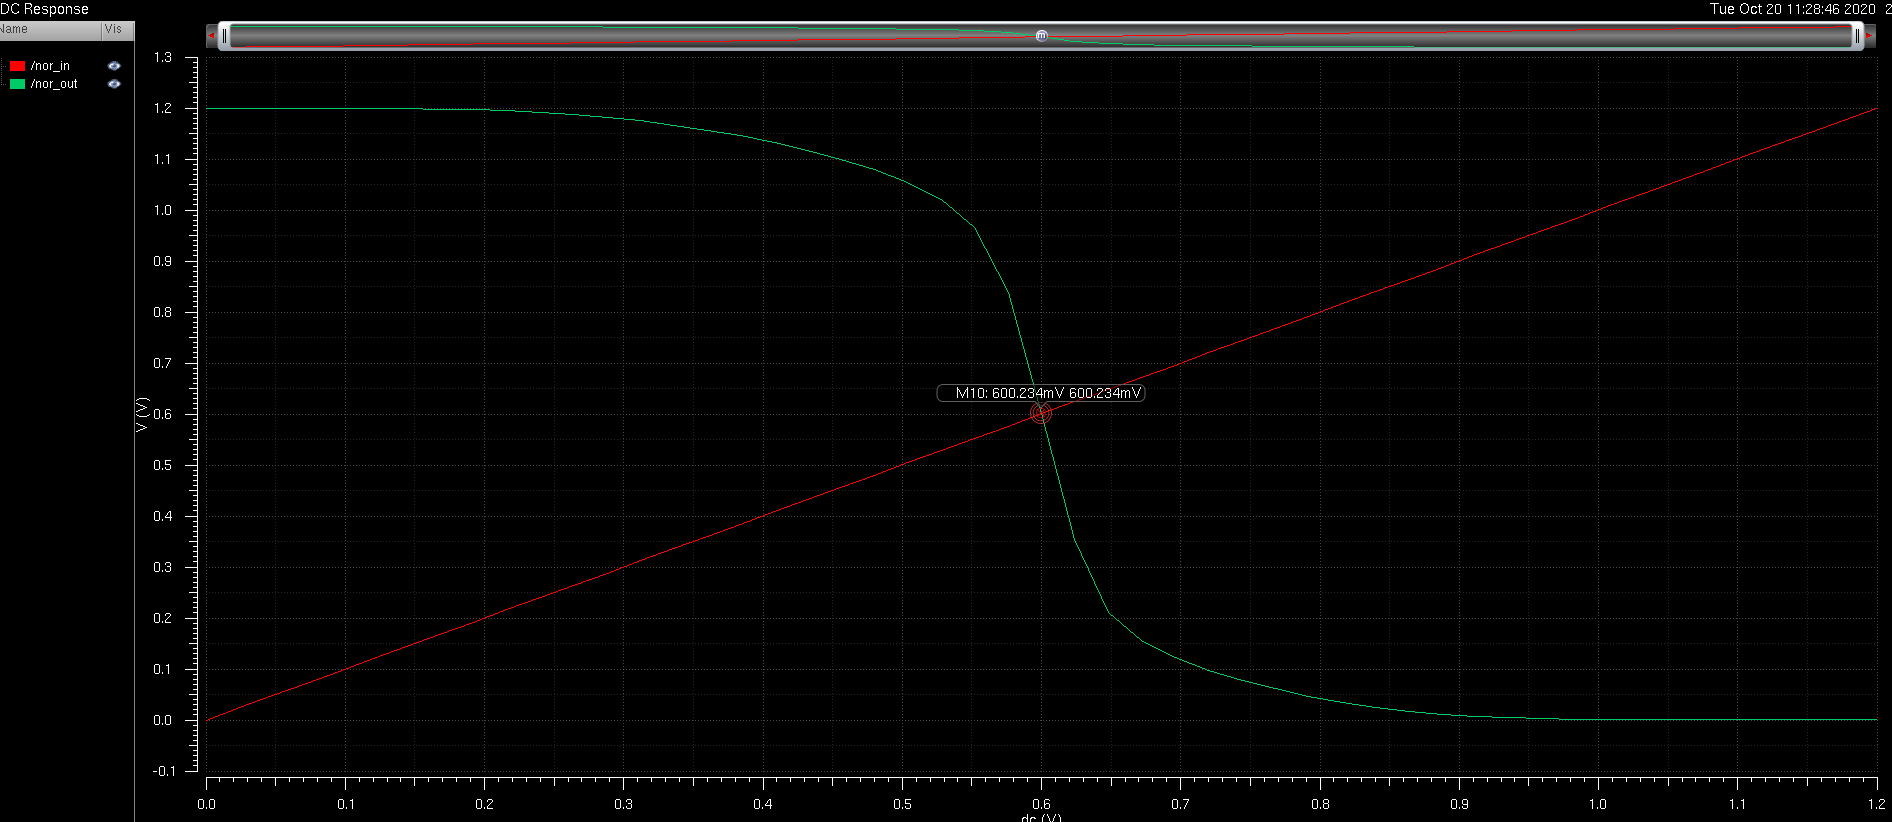
\includegraphics[width=5in]{figures/nor/nor_dc_symm.png}
  \caption{DC Response of a Symmetric NOR Gate}\label{fig:nor_dc_symm}
\end{figure}
\subsection{Layout Design}
After the respective gate's schematic was finished, layout was done. The pmos and nmos were built first, taking special care to make sure the width of the
transistors match the schematic. The pmos and nmos circuits were built first with the Vdd and ground rails being added to the design after as shown in Figure~\ref{fig:nand_layout}.
The same was done for the nor layout and is shown Figure~\ref{fig:nor_layout}.
\begin{figure}[!htb]
  \centering
  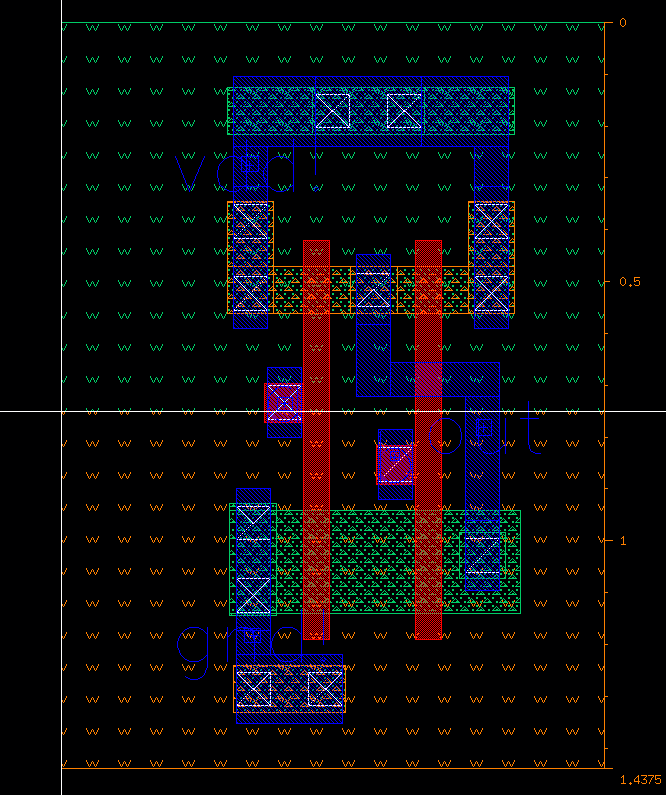
\includegraphics[width=3in,angle=90]{figures/nand/nand_layout.png}
  \caption{NAND Layout}\label{fig:nand_layout}
\end{figure}
\begin{figure}[!htb]
  \centering
  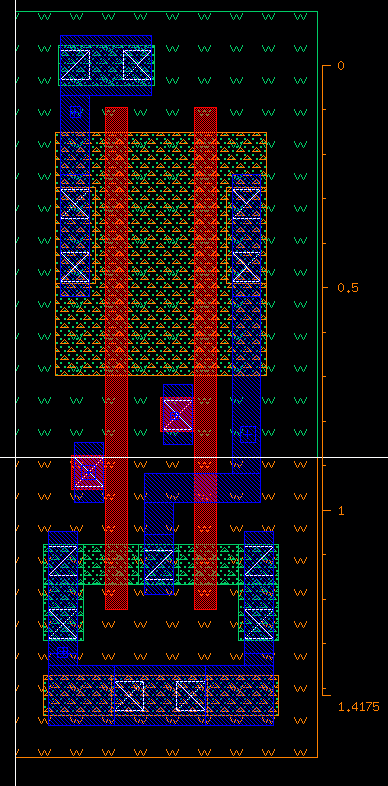
\includegraphics[width=2.5in,angle=90]{figures/nor/nor_layout.png}
  \caption{NOR Layout}\label{fig:nor_layout}
\end{figure}
Lastly, design rule checking(DRC) is used to make sure that no design rules are being violated and everything is fixed very painstakingly. The results for the nand and nor gate can
be seen in Figure~\ref{fig:nand_drc} and Figure~\ref{fig:nor_drc}, respectively  After that layout versus schematic(LVS) was used to make sure our layout matches
the design we modeled with the schematic and can be seen in Figure~\ref{fig:nand_lvs} and Figure~\ref{fig:nor_lvs}, respectively.
\begin{figure}[!htb]
  \centering
  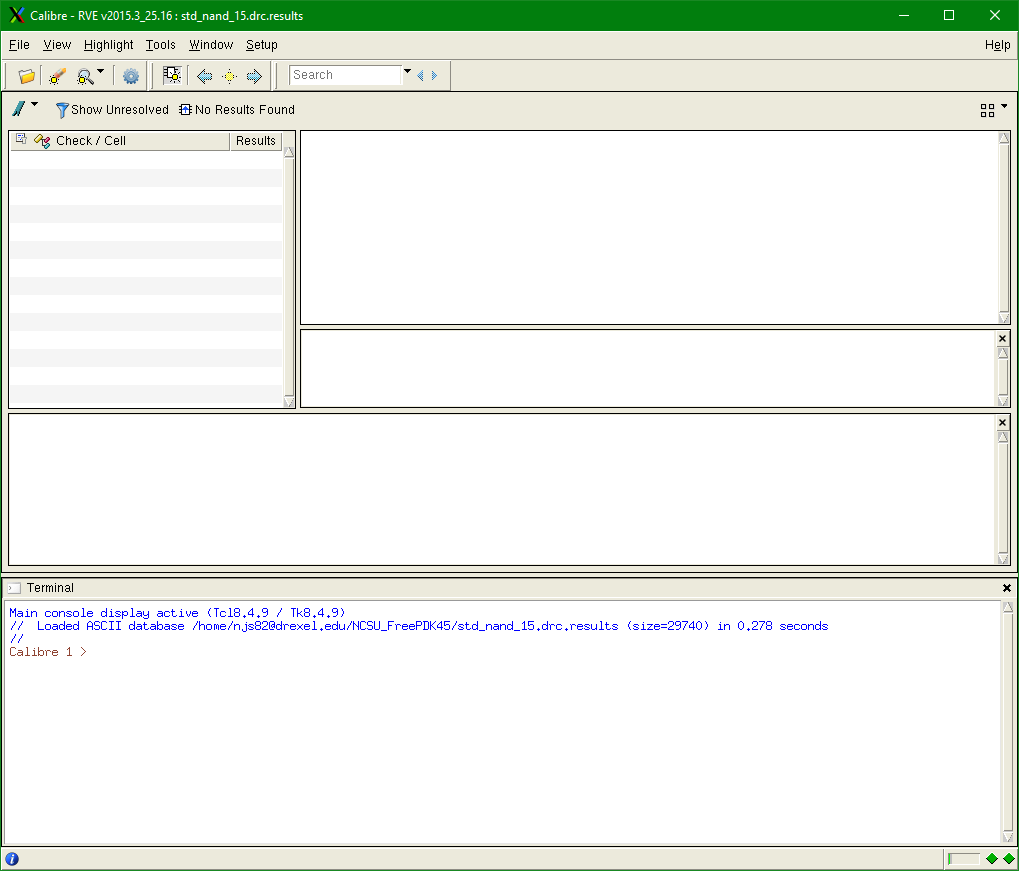
\includegraphics[width=3.5in]{figures/nand/nand_drc.png}
  \caption{NAND DRC Results}\label{fig:nand_drc}
\end{figure}
\begin{figure}[!htb]
  \centering
  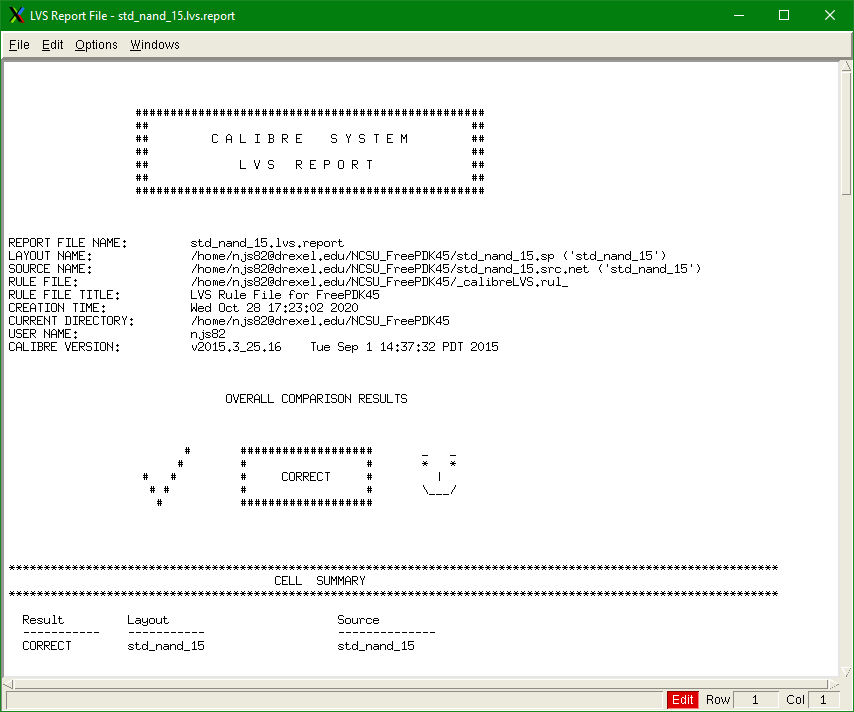
\includegraphics[width=3.5in]{figures/nand/nand_lvs.png}
  \caption{NAND LVS Results}\label{fig:nand_lvs}
\end{figure}
\begin{figure}[!htb]
  \centering
  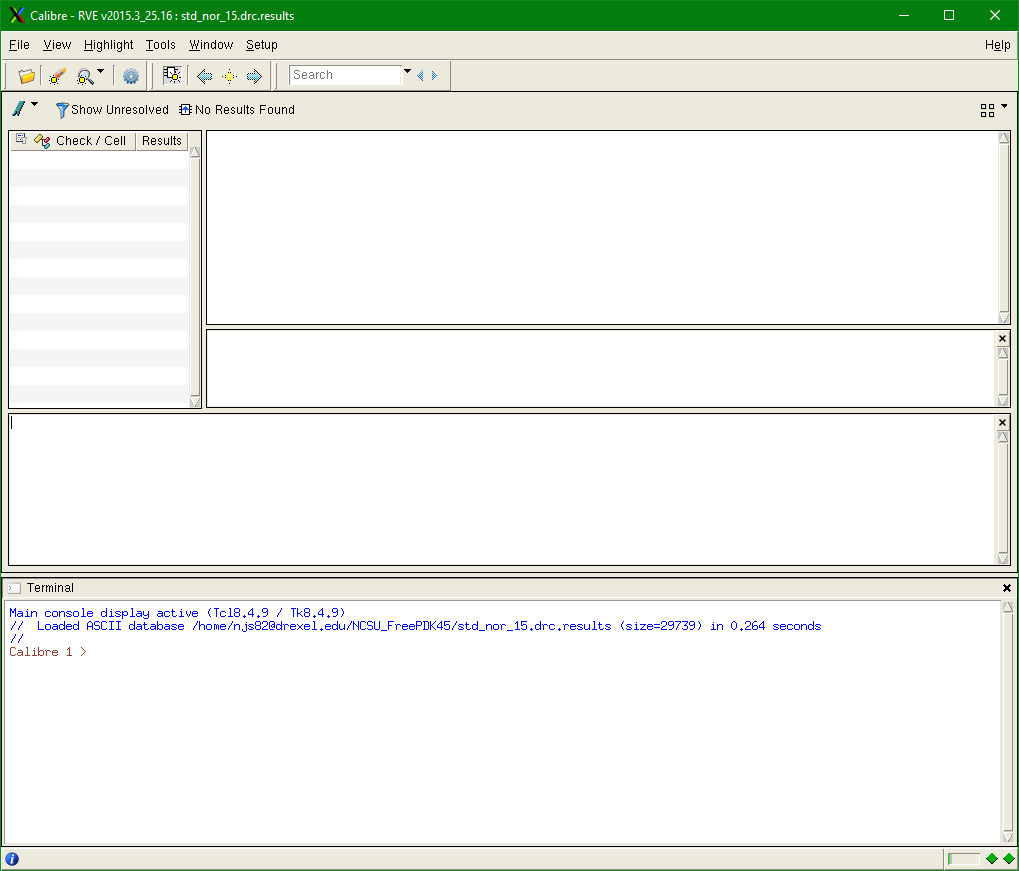
\includegraphics[width=3.5in]{figures/nor/nor_drc.png}
  \caption{NOR DRC Results}\label{fig:nor_drc}
\end{figure}
\begin{figure}[!htb]
  \centering
  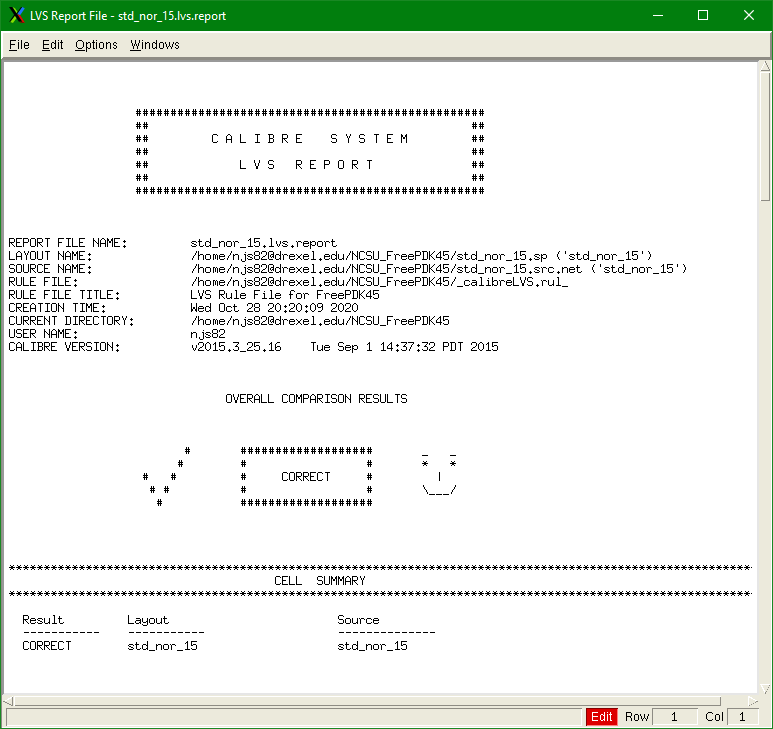
\includegraphics[width=3.5in]{figures/nor/nor_lvs.png}
  \caption{NOR LVS Results}\label{fig:nor_lvs}
\end{figure}
\clearpage
\section{Conclusion}
The lab was a very good way to cement the fundamentals we picked up in lab two by creating two essential gates in any digital designers toolkit.
It helped me further get used to the tools and use them extensively to fine tune my design and make sure everything was working as it should. 
It also helped me get a deeper understanding of the underlying technologies. The only thing I wish I could change is making it easier to find the correct value for a symmetric gate,
which was made a bit easier to tell if the value was correct by the methods we learned in class. Still, though, it is a lot of try, check, and revise to get the perfect value.
\end{document}
%%% Local Variables:
%%% mode: latex
%%% TeX-master: t
%%% End:
